\def\year{2016}\relax
%File: formatting-instruction.tex
\documentclass[letterpaper]{article}
\usepackage{aaai16}
\usepackage{times}
\usepackage{helvet}
\usepackage{courier}
\usepackage{graphicx}
\usepackage{booktabs} % for pretty table rules
\usepackage{hyperref}
\usepackage[T1]{fontenc}


\frenchspacing
\setlength{\pdfpagewidth}{8.5in}
\setlength{\pdfpageheight}{11in}
\pdfinfo{
/Title Wikidata Human Gender Index: An Open Dataset with Perspectives on Times, Space, and Occupation
/Author BLINDED}
\setcounter{secnumdepth}{0}  
 \begin{document}
% The file aaai.sty is the style file for AAAI Press 
% proceedings, working notes, and technical reports.
%
\title{Wikidata Human Gender Index: An Open Dataset with Perspectives on Time, Space, and Occupation}

\author{AUTHORS BLINDED}
    
\maketitle
\begin{abstract}
AAAI creates proceedings, working notes, and technical reports directly from electronic source furnished by the authors. To ensure that all papers in the publication have a uniform appearance, authors must adhere to the following instructions. 
\end{abstract}


\section{Introduction}
The world is rife with inequality offline and on. Wikipedia's editors are largely not women \cite{hill_wikipedia_2013}, and has far-reaching implications into the character of its content. \cite{wagner_its_2015} showed that while coverage of women in large Wikipedias is not worse than other references, the language with which women are portrayed is different and focuses more on romance and family. Additionally they are less central in the internal graph of Wikipedia. These linguistic and network findings were confirmed by \cite{graells-garrido_first_2015}, who also showed evidence of stereotyping in metadata. Yet in popular mindshare there persists a sentiment that denies that any of this is a problem \cite{eckert_retriggering_2013}. Luckily, experiments have shown that awareness of Wikipedia's gender issues is a strategy that can alleviate the problem \cite{hinnosaar_gender_2015}, for which more methods are always needed.

Wikidata, the database that feeds Wikipedia, offers new opportunities to analyze culture programmatically through. Launched in 2012, Wikidata is designed to host structured data that is multilingual (easily translatable so there is only one edition), and plural (can support many competing facts) \cite{vrandecic_wikidata:_2014}.  These features make Wikidata the perfect place for all Wikipedias to to collaboratively store facts about the world. If an Italian Wikipedian stores information about the population of ancient Rome, that information is then available to every other Wikipedia with a short code snippet. Every language collaborating together has meant that Wikidata has become a massive free open knowledgebase in its own right, containing over 40 million facts \cite{krotzsch_how_????}.

As a knowledgebase Wikidata is slowly proving its worth for research. For instance, Wikidata has been used to find popular connections between nationalities and occupations \cite{goldfarb_quantifying_2015}. Or take the fact that all human and mouse genes have been imported into Wikidata \cite{mitraka_wikidata:_2015}, for an internet-wide community effort to find links between genes, drugs and diseases \cite{burgstaller-muehlbacher_wikidata_2015}. All of these tasks would be difficult to do without Wikidata.

We introduce a weekly-updating dataset called the ``Wikidata Human Gender Index'' (WHGI), which measures the gender of the humans represented in Wikidata - that is, Wikipedia biography articles - across time, space, and occupational dimensions. Measuring and releasing data on Wikipedia's content gender gap attempts to solve two problems. The first is to shed light on the problem under the philosophy of ``what gets measured, gets fixed.'' Perhaps even more excitingly though, the scope of Wikidata gives us an unprecedented look at gender through time, space, and occupation, at a scale never seen before, which has potential applications for a not-possible-until-now open data mashups.

This paper begins by describing the format of the data presents a variety of statistics to illustrate how to use the data. We investigate how the data quality has changed over time, which demonstrates the 9 semantic properties available, and the advantages of its weekly, ``snapshot'' feature. We produce a top-10 of Wikipedia's which increased in their female ratio of human biographies as a example problem. 

To show that WHGI is not a not entirely Wikipedia navel-gazing, we present 3 validation measures utilizing ground truths from the US Census Bureau, Bureau for Labor Statistics, and United Nations Development Program. We show that the WHGI does in fact relate to the real world. This means that, albeit imperfectly, the WHGI can be a proxy for numerical data about the real word in times and places for which no previous data exists.

Finally, the WHGI is meant for re-use, and we present some potential applications, and scenarios for which it could be used in historical and linguistic research.  

\section{Dataset Details}

\begin{figure}
\label{fig:screenshot}
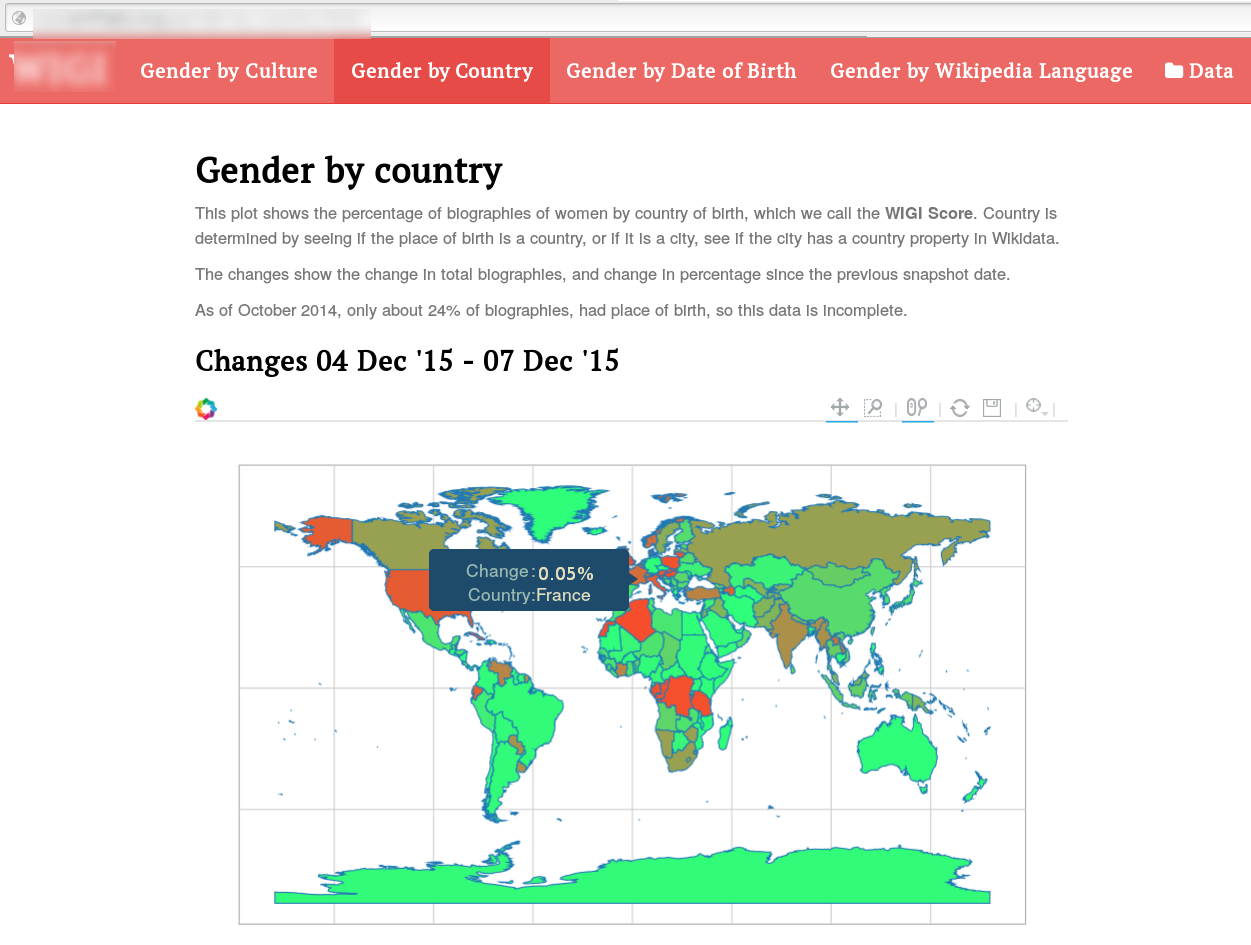
\includegraphics[scale=0.2]{figures/website_screenshot.png} 
\caption{Screenshot of WEBSITE BLINDED displaying the gender by culture plot.}
\end{figure}

Our dataset is available for free under the CC-BY-SA license online at  \url{WEBSITE BLINDED}. Here a visualization demonstration of our data lives, and direct downloads, from the \url{WEBSITE BLINDED/} folder. 	This folder contains the CSV-formatted, weekly captured \textit{snapshots} of gender-related data from Wikidata. Each snapshot contains an unaggregated one-row-per-human complete view of the data, \textit{aggregated} ``property''-specific files, aggregated by tempo, spatial, and other properties, and weekly changes between the property indexes. Our first snapshot is from September 17\textsuperscript{th} 2014, the latest presented here is January 3\textsuperscript{rd} 2016, but snapshotting is automated and tracks the official Wikidata data dumps.

\subsection{Processing}
Each week, just after the release of Wikidata's official weekly data dump, we download a copy of the dump and process it in the following way. Using the Wikidtata Toolkit \footnote{\url{https://www.mediawiki.org/wiki/Wikidata_Toolkit}} the entire database is subsetted to only those items which have the property \textit{instance of} with value \textit{human} - or ``P31:Q5'' in Wikidata terms.

For each human item we find the values of \textit{gender}, \textit{date of birth}, \textit{date of death}, \textit{place of birth}, \textit{citizenship}, \textit{ethnic group}, \textit{field of work}, and \textit{occupation}. These correspond to Wikidata properties P21, P569, P570, P19, P27, P172, P101, and P106 respectively.  In every snapshot folder this complete list of humans is saved as ``gender-index-data-\{snapshot data\}.csv'', it records one Wikidata item per row, and it's columns are the value of each property. 

Because Wikidata is multilingual its values are stored as identifiers, which every language can translate. To maintain fidelity we keep this standard, so for example Aung San Suu Kyi represented in Wikidata in English looks like Figure \ref{fig:aung} and in our dataset would be a row like \begin{small} Q36740,1945,,Q6581072|,,Q836|,Q37995|,,Q82955|Q36180|Q1476215|
\end{small}. Our code examples include functions to translate these Q-IDs into English labels.

\begin{figure}
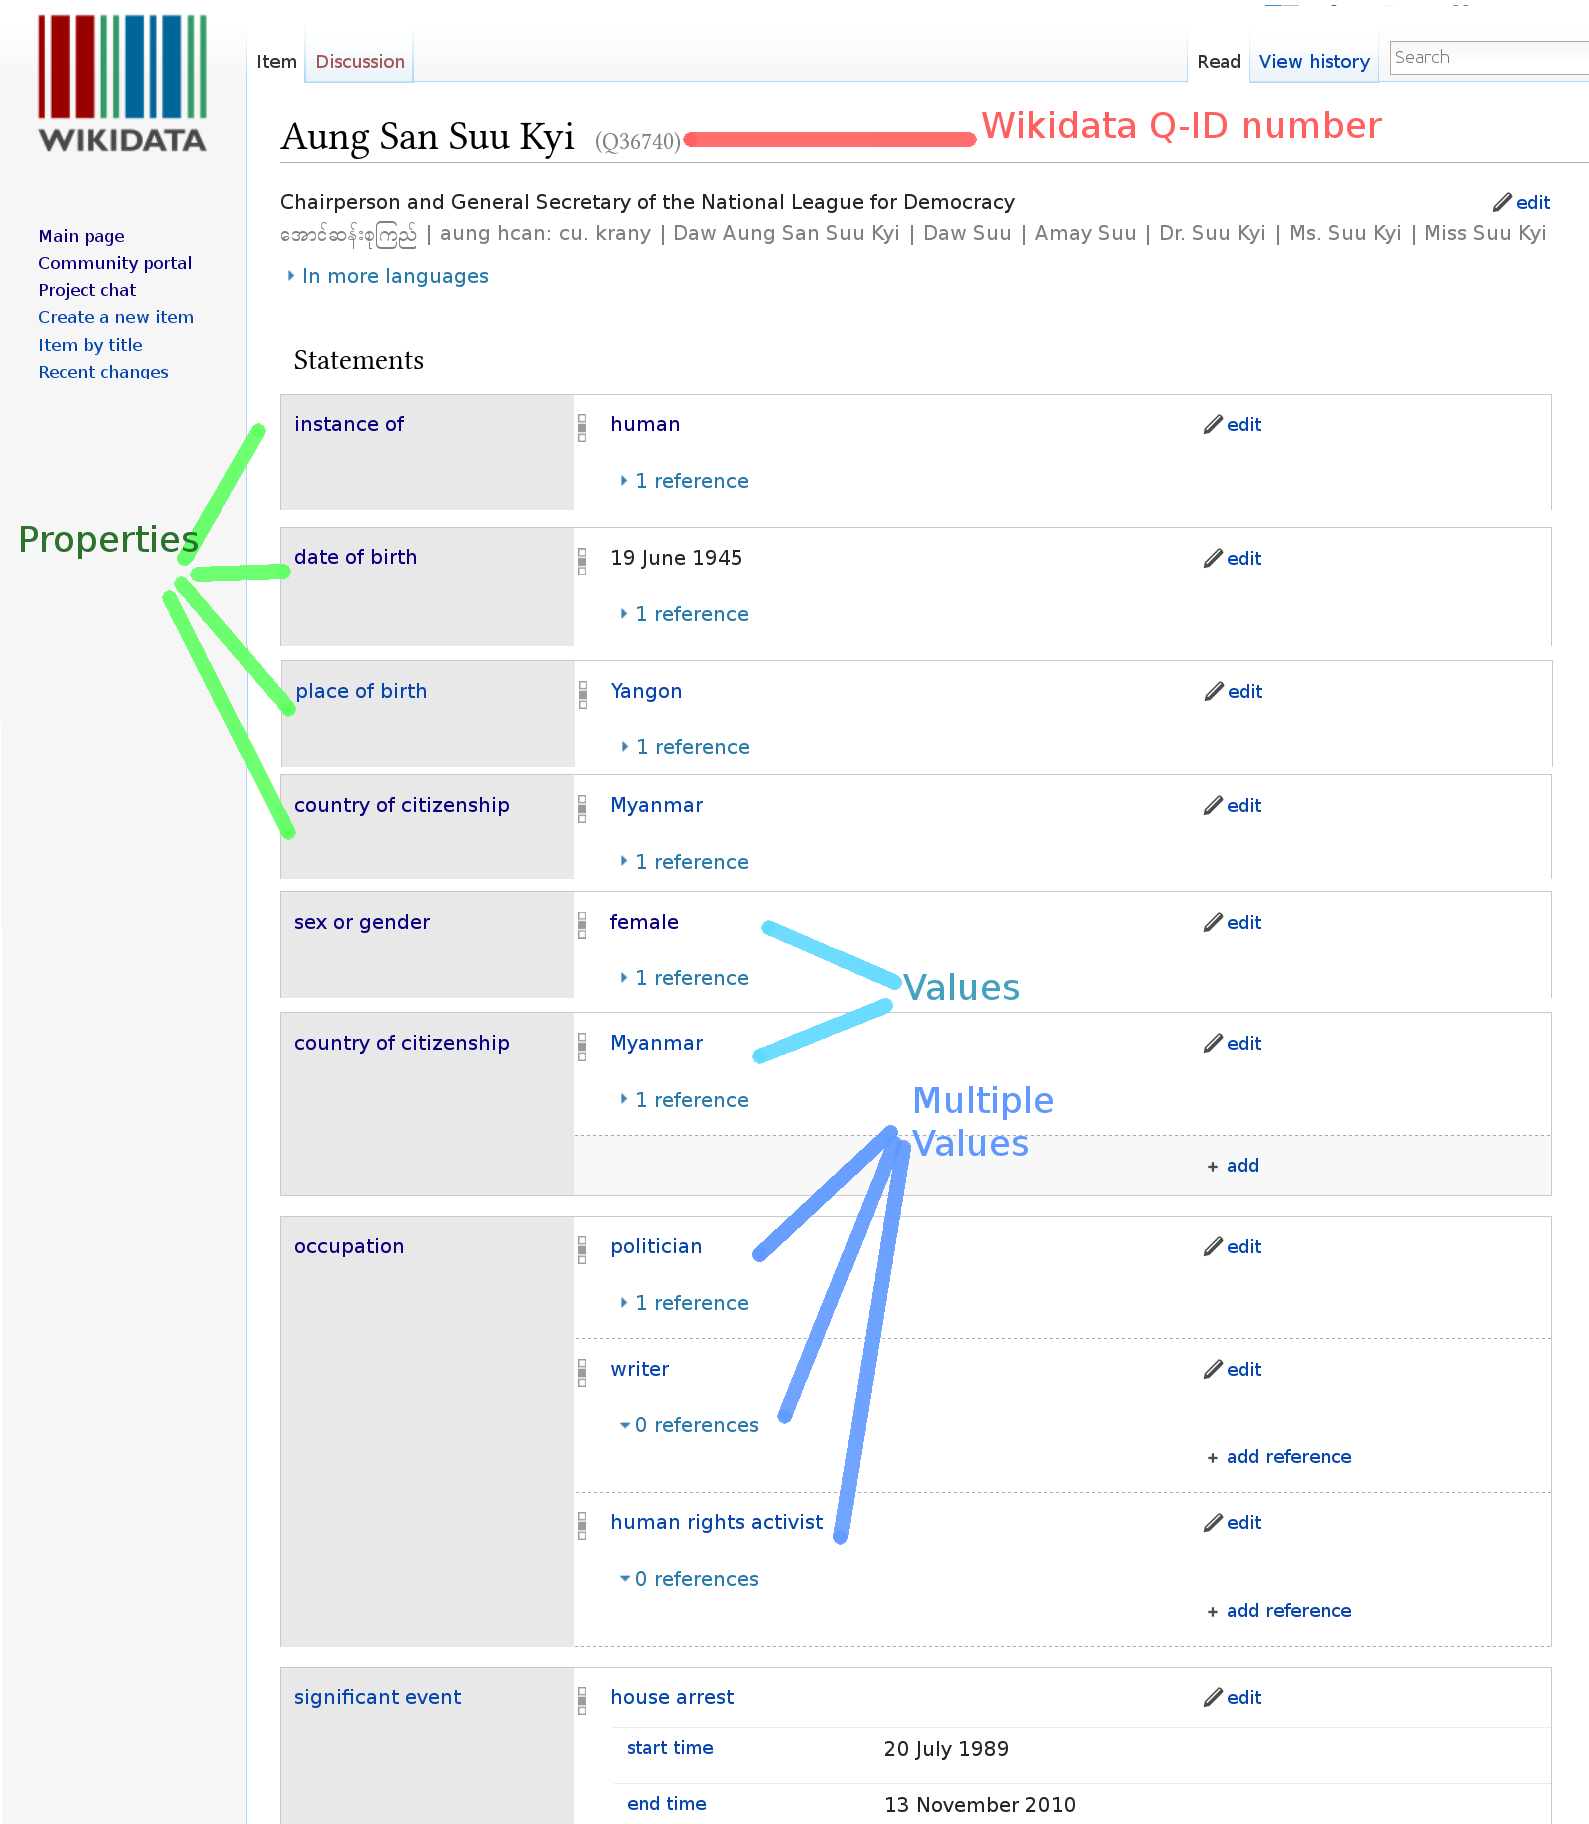
\includegraphics[scale=0.15]{figures/aung_explainer.png} 
\caption{Example Wikidata Human Item of Aung San Suu Kyi}
\label{fig:aung}
\end{figure}
 
For each of the recorded properties we then aggregated the dataset on that property, but disaggregated by gender. Take for example the date of birth file. it has one row per year unique year found as a date of birth, and one column per gender represented in Wikidata. See a sample excerpt from the in the January 3\textsuperscript{rd} 2016 snapshot in Table \ref{table:dob}. Additionally there is an aggregate on the Wikipedia languages in which a human is represented - \textit{sitelinks}, and a geographic aggregation of citizenship, place of birth and ethnic group into properties called \textit{culture}, and \textit{worldmap}. Inside every snapshot folder there exists a subfolder titled ``property-indexes'' containing 11 aggregates of the snapshot - one per property dimension.
 
\begin{table}
\caption{Excerpt of the 2016-01-03 date of birth-aggregate file. N/A are humans without recorded gender.}
\begin{tabular} {p{0.8cm}p{0.8cm}p{0.8cm}p{0.8cm}p{0.8cm}p{0.8cm}p{0.8cm}}
\toprule
date of birth & no gender & trans-gender female & gender-queer & ka-thoey & female & male \\
\midrule
1980 & 839 & 2 & 1 & & 5,092 & 14,137   \\ 
1981 & 849 & 1 &  & 1 &5,042 & 14,461 \\ 
1982 & 861 & 2 &  & &5,132 & 14,372  \\ 
1983 & 864 & 3 &  & &5,078 & 14,520  \\ 
1984 & 830 & 3 & 1 & &5,372 & 14,558   \\ 
1985 & 777 & 4 &  & &5,400 & 14,664  \\ 
\bottomrule
\end{tabular}
\label{table:dob}
\end{table}

The third item in every snapshot folder is titled ``changes-since- \{previous snapshot date\}, and contains computed differences between this snapshot and the last. This feature allows inspection of the movements of the past week. There is one changes-since file for each property file. Using the date of birth example again, the changes-since file will show which genders were added - or subtracted - for each year, in the course of the week.

Examples of how to process the CSVs and generate the following results using both \textit{python-pandas} and \textit{R} can be found in our github repository \footnote{\url{WEBSITE BLINDED}}.

\subsection{Online Visualization}
As a demonstration our website displays 4 interactive visualizations of the dataset. Figure \ref{fig:screenshot} shows the \textit{gender-by-country} visualization, which shows the female ratio of humans by place of birth and citizenship combined during the past week. Figure \ref{fig:screenshot2} shows the \textit{gender-by-language} visualization which compares the female ratio of biography by Wikipedia language, for the entirety of the dataset - ``all time''. The visualizations are interactive which allow the user to investigate specific parts of the plots. Each visualization is available both for all time, and the previous week. We also produce top-10 information for each plot for readability. The remaining 2 unmentioned visualizations are \textit{gender-by-culture}, where culture is a further aggregation of countries and \textit{gender-by-date-of-birth-and-death}.

\begin{figure}
\label{fig:screenshot2}
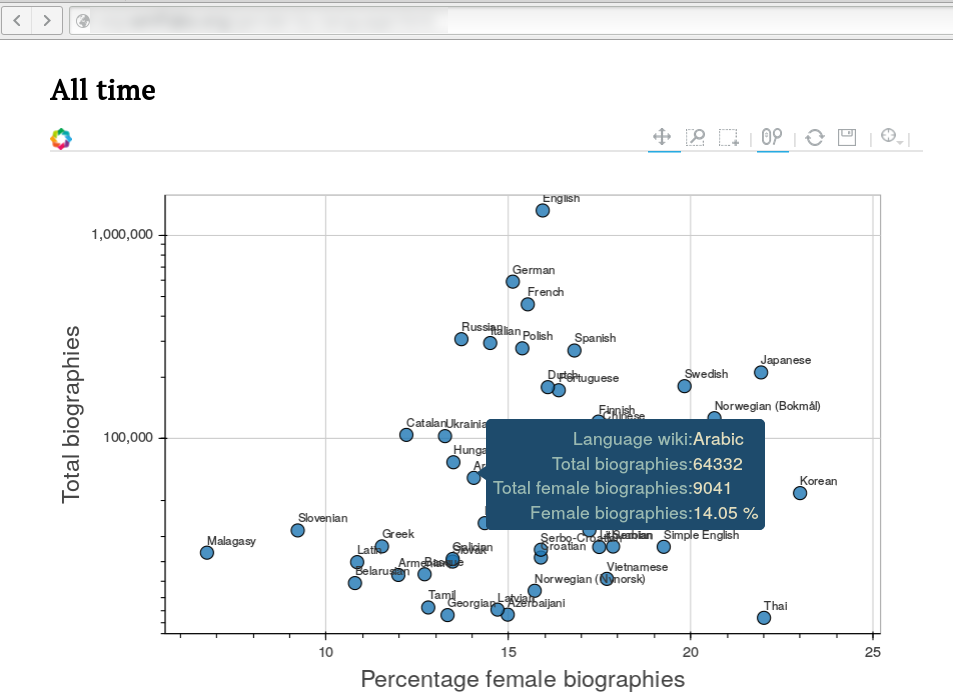
\includegraphics[scale=0.25]{figures/screenshot2.png} 
\caption{Screenshot of WEBSITE BLINDED displaying the gender by language plot.}
\end{figure}

Finally there are two special folders in our root directory which we offer for convenience,  titled \textit{newest} and \textit{newest-changes}, which will always link to the most recent snapshot, and the changes between the two most recent snapshots (week to week), respectively. This makes it easy to always access the freshest data.

\subsection{Technical Details}
In order to faithfully represent Wikidata, the value of each property is actually a list, since Wikidata allows there to potentially be multiple values for a property. This is because either two sources disagree on a property, or like in the case of Aung San Suu Kyi, she has many occupations \ref{fig:aung}. We store the list, inside the comma-separated sheet, as | ``pipe''-separated values. Of course these multiple values introduce a design problem in aggregating on a list of properties. Our method is to aggregate on the list, rather than on the individual items within the list. This means in the case of Aung San Suu Kyi, that her occupation is stored as politician, writer, and human rights activist, and is aggregated with all the other humans who have those three occupations too.

Also note, for faithfulness there is virtually no data-cleaning done, as the point of our project is to display information as faithfully as possible. Our dataset is meant to be used to uncover potential biases in Wikidata and the world at large, and we feel that any cleaning process would introduce further biases. An instructive illustration of this case is that the ``gender'' property in Wikidata is actually labelled in English ``sex or gender'' (no distinction), and not limited to any value. Over our time snapshotting we found 36 values used for ``sex or gender'', including ``male'' and ``female'', but extending to nonbinary genders ``transgender female'', ``intersex'', ``fa'afafine'', ``transgender'', ``Gender fluid'',  ``genderqueer'', ``kathoey'', and ``queer''. At times the other categories of information is recorded here - perhaps erroneously - such as ``gay'', or ``homosexuality''. And even what seem to be mistakes are left in such as one-offs of ``Solanum tuberosum'', ``Messi'', or ``sociologist''. Cleaning this data would be a disservice, we feel, to communicating how - and how well - Wikidata is used.

\section{Dataset Statistics}
We now turn to look at simple statistics of our dataset, specifically with regard to how it has changed over time. Our first snapshot was on September 17\textsuperscript{th} 2014, and the latest analysed here is January 3\textsuperscript{rd} 2016. Since automation of snapshotting was not completed until June 28th 2015, there is unfortunately a window missing from October 2014 to June 2015. 

\subsection{Data Quality}
Let us first query the size of the dataset. Total humans in Wikidata increased from 5,869,606 to 6,999,542, and shows linear, unconstrained growth (see Figure \ref{fig:totalhumans}).

\begin{figure}
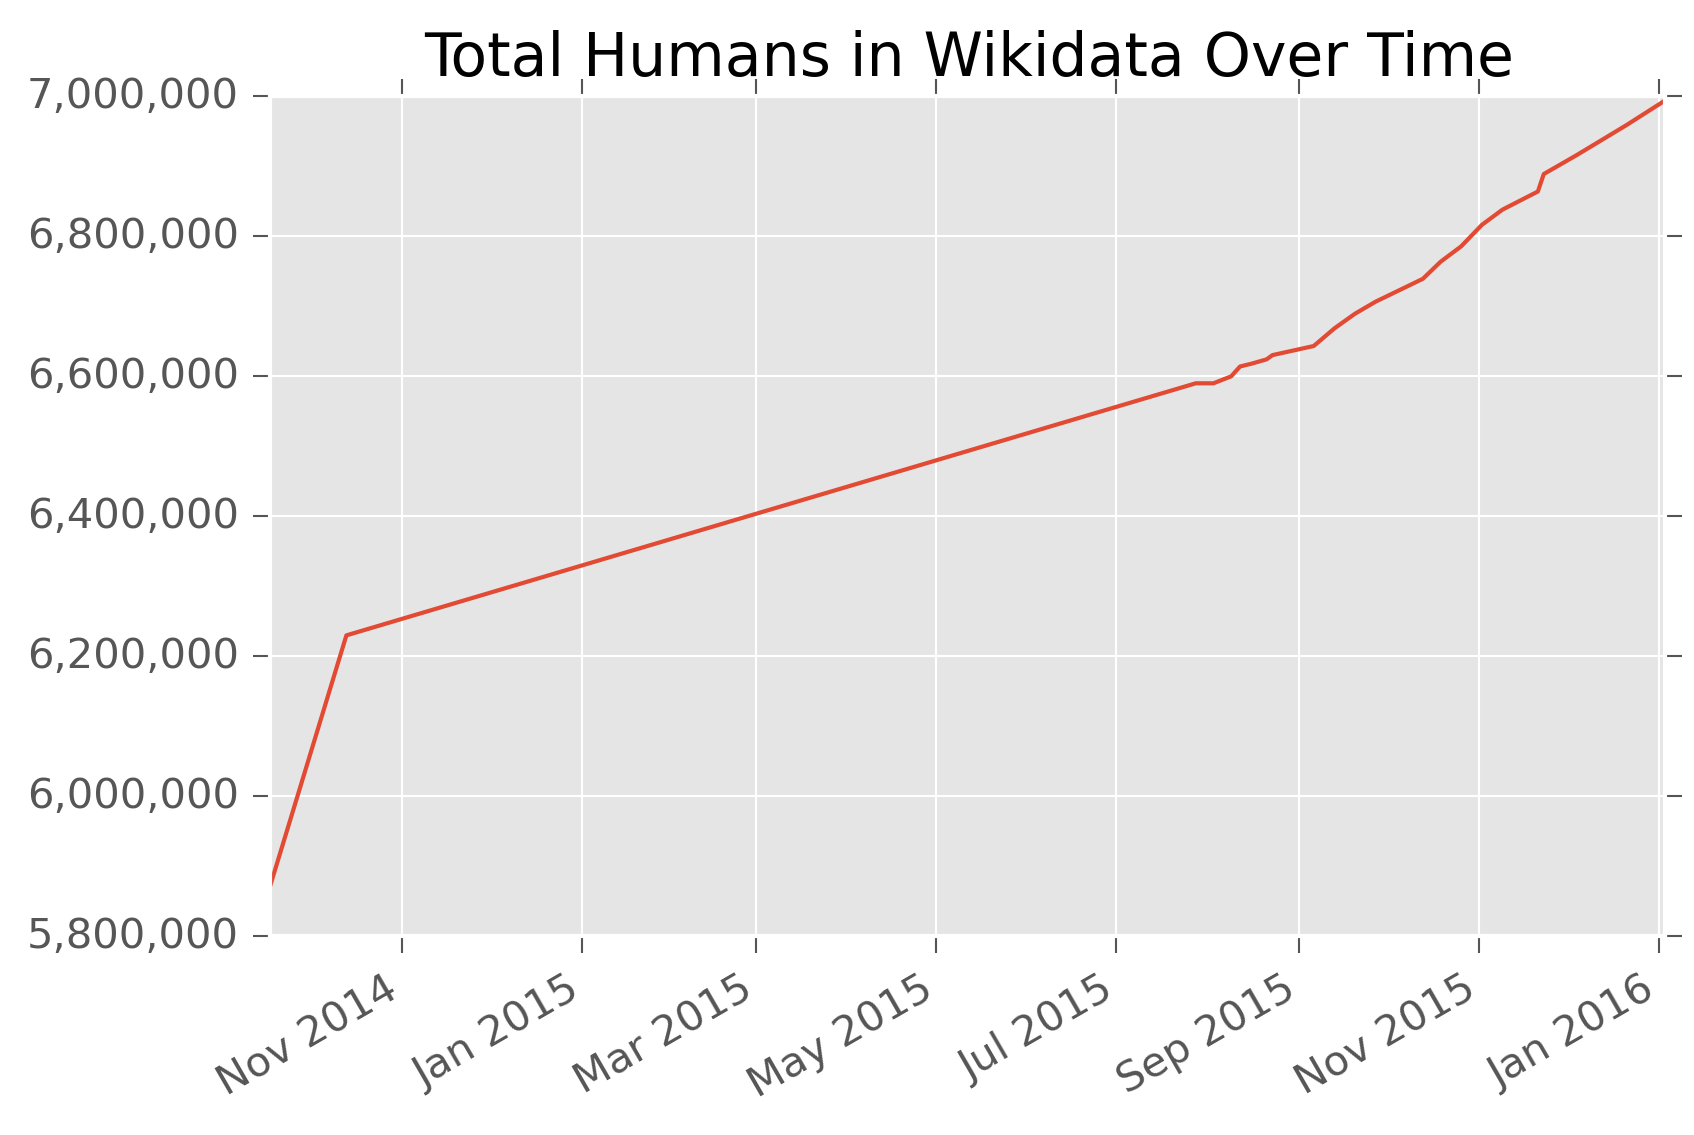
\includegraphics[scale=0.6]{figures/totalhumans.png} 
\caption{Total number of humans found in Wikidata at each snapshot period.}
\label{fig:totalhumans}
\end{figure}

\begin{table}
\caption{Change in rates of property coverage for humans}
\begin{tabular}{lrr}
\toprule
{} &  2014-09-17 &  2016-01-03 \\
\midrule
gender               &       95.3\% &       96.5\% \\
date of birth        &       57.6\% &       71.7\% \\
date of death        &       28.6\% &       36.1\% \\
citizenship          &       42.8\% &       58.2\% \\
place of birth       &       24.0\% &       30.5\% \\
ethnic group         &        0.3\% &        0.6\% \\
field of work        &        n/a &        0.3\% \\
occupation           &        n/a &       58.7\% \\
at least 1 site link &       99.6\% &       98.1\% \\
\bottomrule
\end{tabular}
\label{table:accompanying}
\end{table}

We should also be curious to the data quality of the increasing humans. One way to think about this coverage of properties on these human items. We investigated the coverage completeness for all  properties we recorded. Another mark of quality is whether a human in Wikidata has an entry in a Wikipedia - a ``sitelink'' in Wikidata vocabulary. Figure \ref{fig:accompanying} shows the trend in coverage of properties from the earliest and latest snapshots from 2014 and 2016 respectively. The statistics show that data quality has been increasing almost uniformly over time. The number of humans with \textit{gender} data increased by over 1\%, closer to complete coverage. In the time domain \textit{date of birth} and \textit{date of death} coverage increased by 14\% and 7\%. Likewise \textit{citizenship} data increased by 15\%, \textit{place of birth} by 6\%, and \textit{ethnic group} almost doubled (see Table \ref{table:accompanying}). \textit{Field of work}, and \textit{occupation} data was not included in our dataset until late, so their growth, while increasing is not precisely comparable.

Curiously the rate of humans having sitelinks decreased slightly, but this is which has an important interpretation. A Wikidata human without a Wikipedia article is know as a ``structural item''; for instance a member of royalty without a Wikipedia article but is a needed to make a family tree complete. With the view that a structural item is an artefact from humans paying attention to Wikidata's structure, the decrease in sitelinked humans can also be seen as a rise in data quality. Probably there are also biography articles in Wikipedias that are not semantically described as humans in Wikidata, however this set is difficult to enumerate since knowing that a Wikipedia article is about a human is difficult to do programmatically. 


\begin{figure}
\label{fig:accompanying}
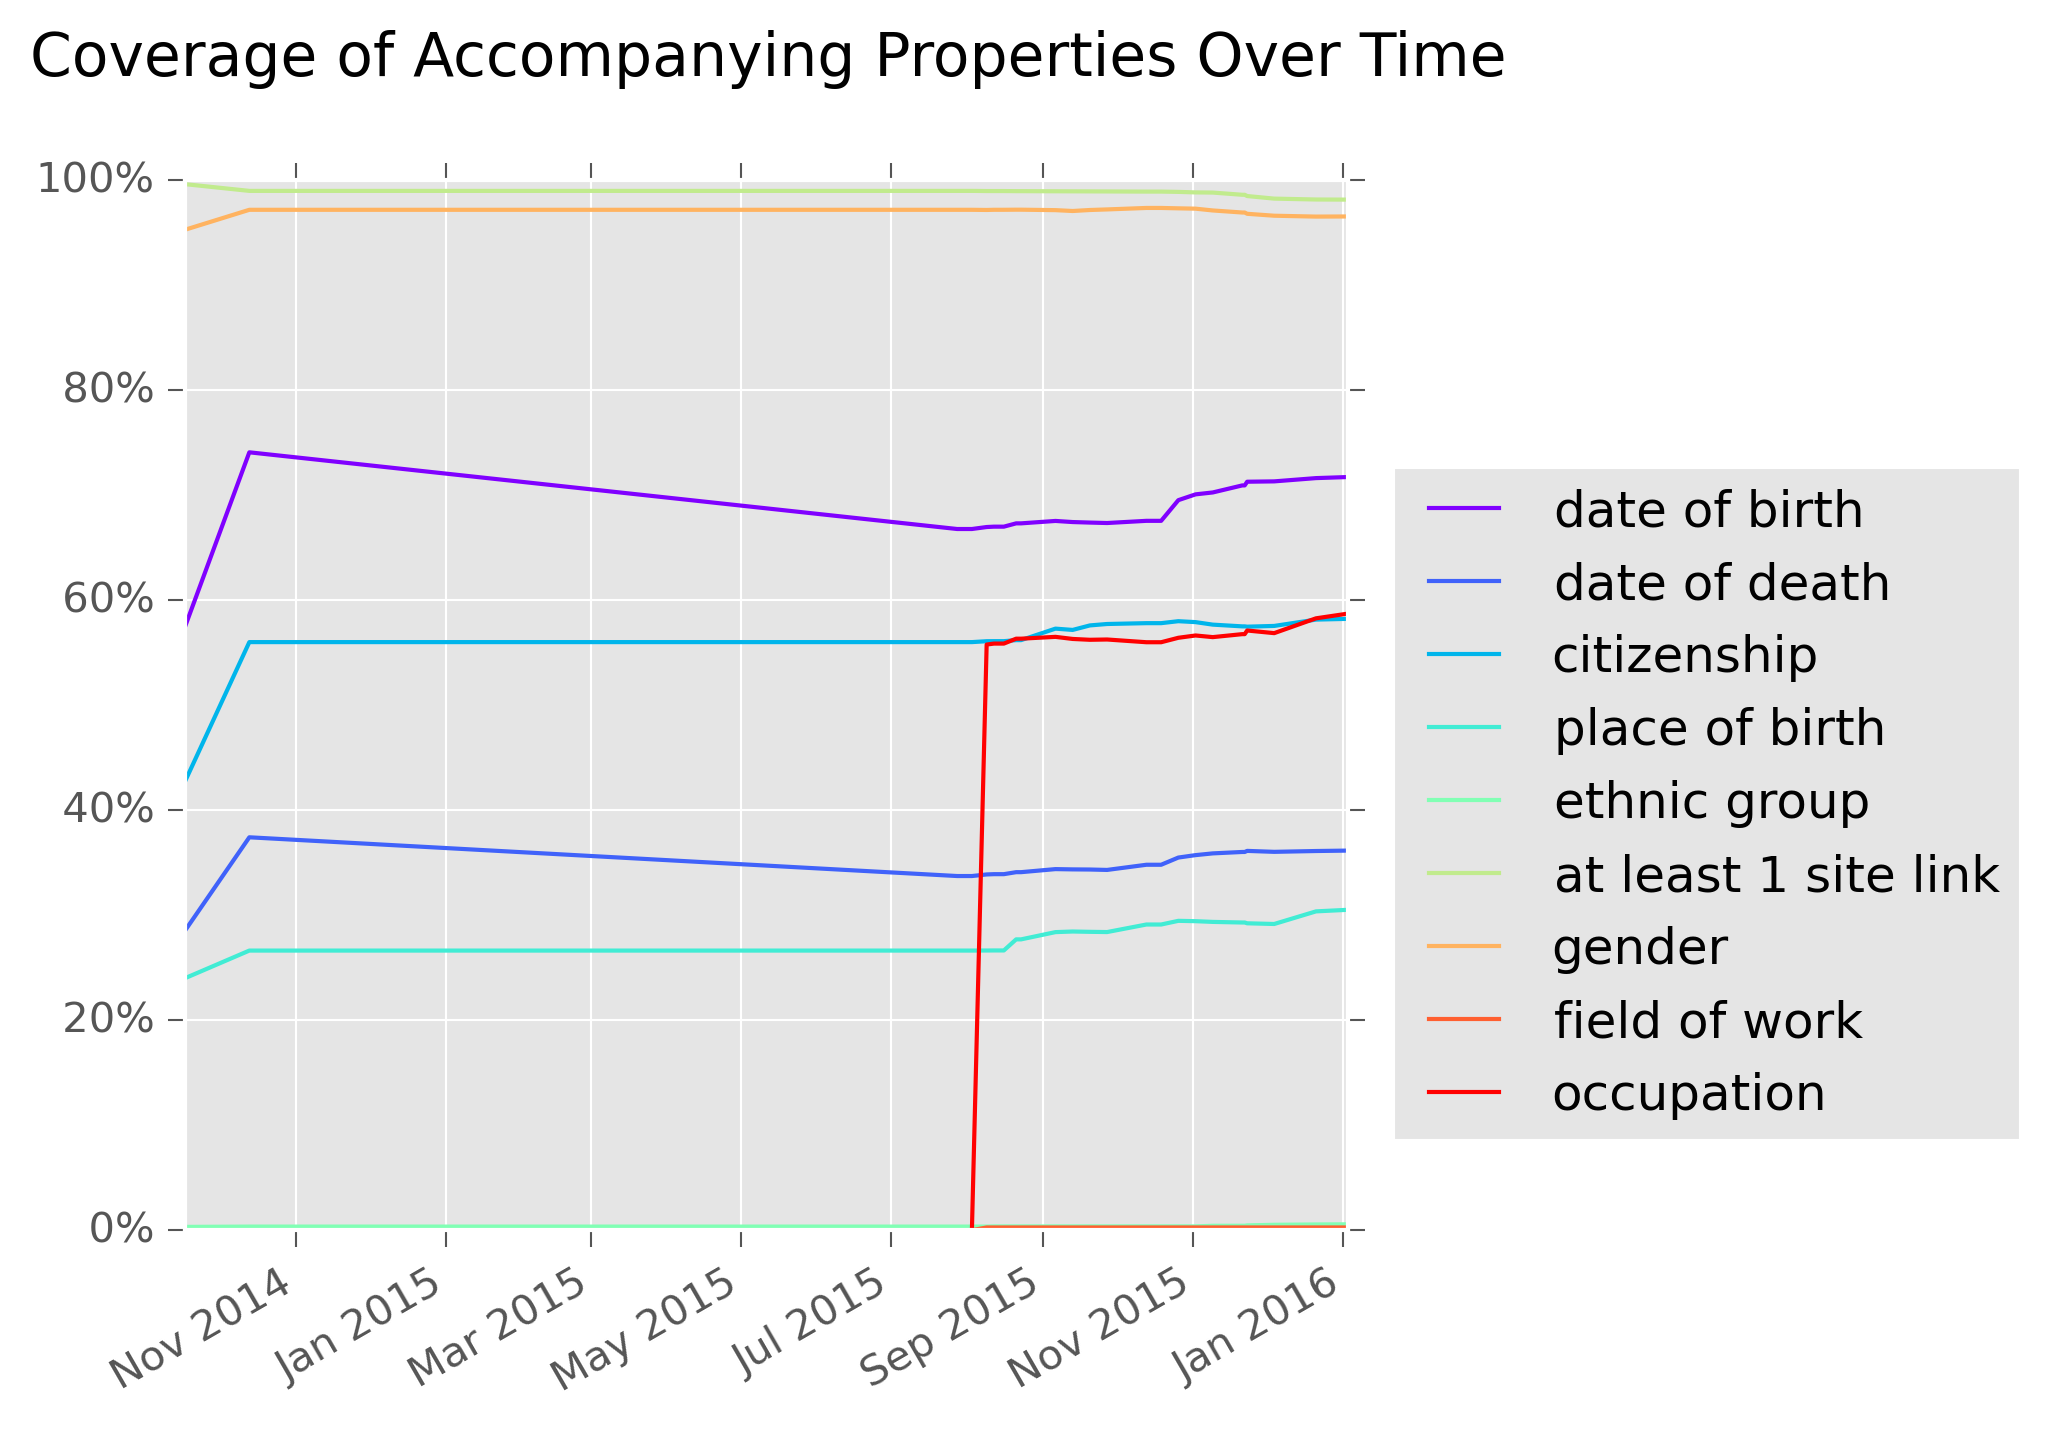
\includegraphics[scale=0.5]{figures/additionalprops.png} 
\caption{Trend of human-accompanying properties by snapshot.}
\end{figure}

\subsection{Simple Metrics}
As further motivation for how the dataset can be used, we present some simple metrics which would be of interest to Wikimedian communities. Focusing on one of our motivations, monitoring the trend of gender representation, we inspect the rate at which women are recorded in Wikidata. Figure \ref{fig:frb} shows the ratio of ``female'' recorded humans versus all gendered biographies. Similarly to total biographies this measure is rising at a fairly linear rate of approximately 0.5\% per year. The final months on record show a slight decline which warrants further investigation. In fact being able to measure at this temporal level is precisely one of the points of having such a live-updating measure - to be able to detect trends as they happen, and perhaps relate them to community issues. 

\begin{figure}
\label{fig:frb}
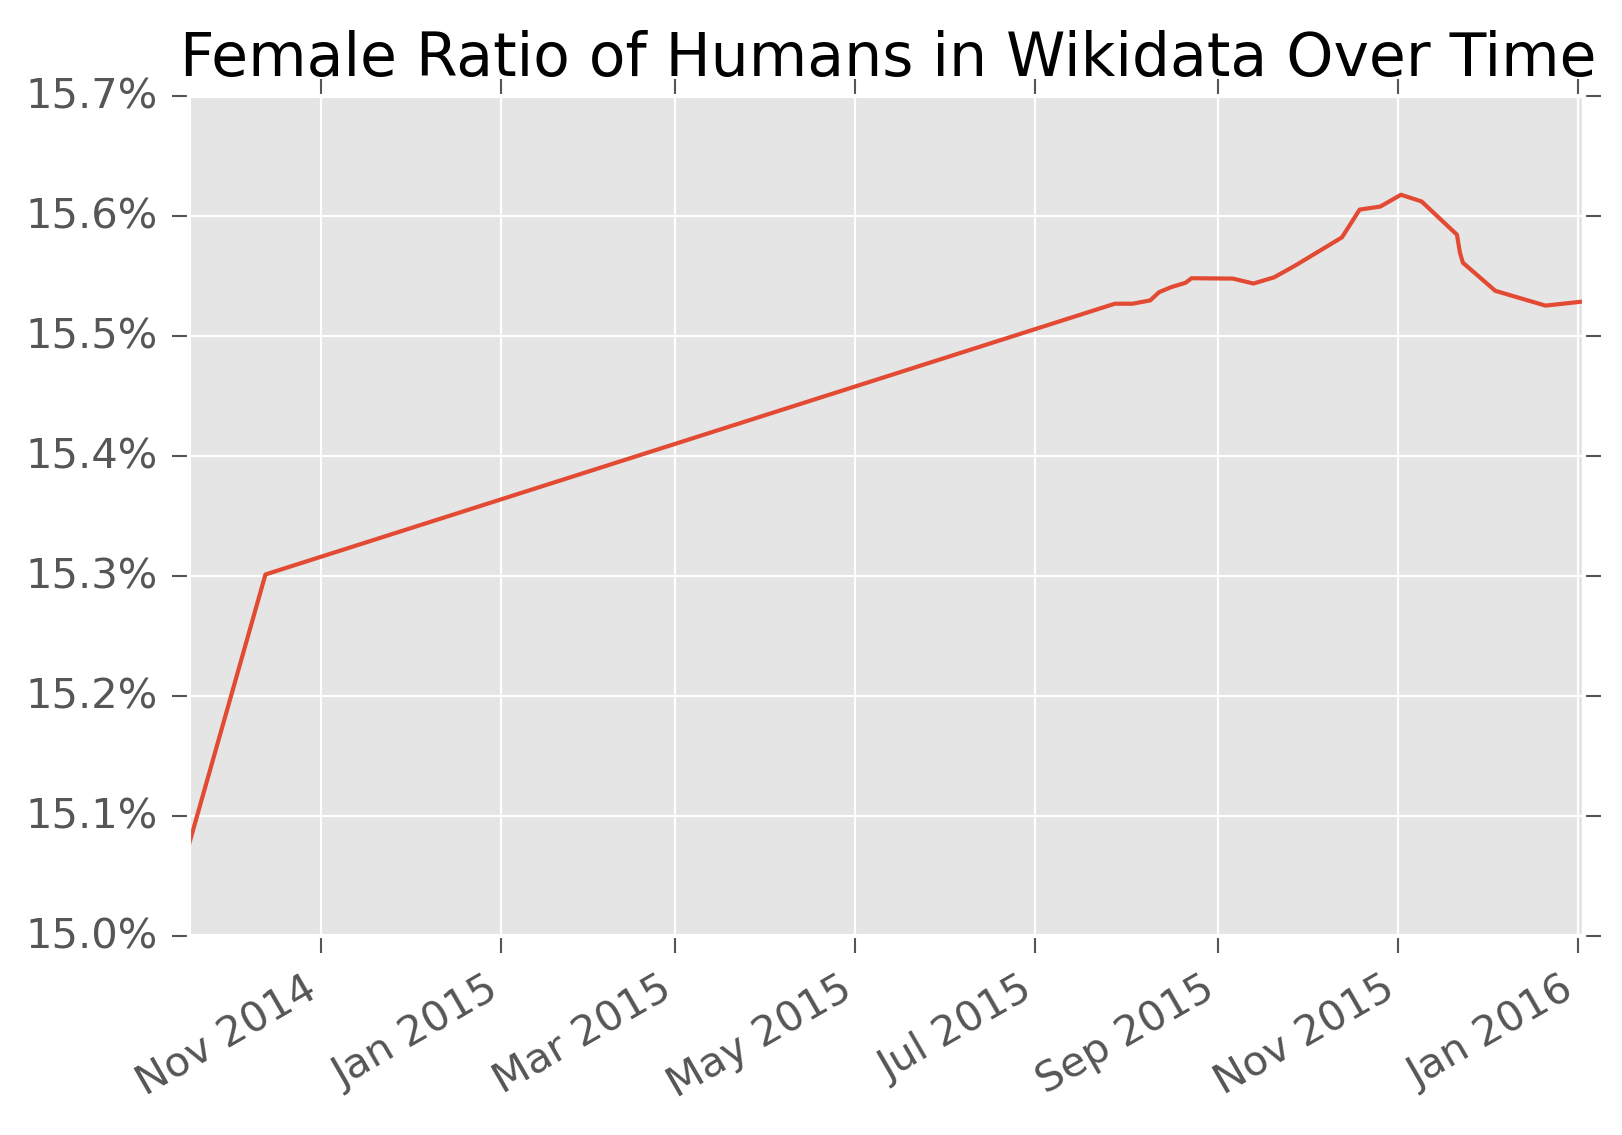
\includegraphics[scale=0.6]{figures/frbwikidata.png} 
\caption{Trend of human-accompanying properties by snapshot.}
\end{figure}

Another way in which Wikimedians can use the data is to look at trends specific to Wikipedia languages. It is easy to use the data to compile a top-10 list of Wikipedias whose female ratio of humans increased the most, see Table \ref{table:top10} This measure does not explain whether women's representation in those languages increased because because editors took longer to record women's gender in Wikidata and were catching up in the observed period, or that these languages became more women-focused over the snapshotting period. Such forensics is possible with this dataset though.

\begin{table}
\caption{Top 10 Wikis by increase in female ratio of humans from October 2014 to January 2016}
\label{table:top10}
\begin{tabular}{p{2cm}p{2cm}}
\toprule
{Wiki} &     Increase in female ratio of humans  \\
\midrule
Lithuanian      & 5.31\% \\
Japanese     & 4.76\% \\
Estonian      & 4.58\% \\
Slovenian      & 2.19\% \\
Tagalog      & 1.63\% \\
Korean      & 1.38\% \\
Finnish      & 1.33\% \\
Wikimedia Commons & 1.20\% \\
Farsi      & 1.17\% \\
Hebrew      & 1.17\% \\
\bottomrule
\end{tabular}


\end{table}

\section{Validation}
In order to gain an idea about how well WHGI reflects the real world, we validated out data by comparing it against 3 exogenous datasets. We correlated the WHGI date of birth frequency versus historical world population trends; WHGI gender by country versus external by-country gender-disparity indexes; and WHGI occupation by gender versus United States Bureau of Labor Statistics occupation gender.

\subsection{World Population} Our most simple validation measure involved comparing the world's population by year to the number of humans in WHGI by year of birth. We conduct this validation even though, the number of people alive and the number of Wikipedia-notable people born are different measures. However if we operate under the assumptions that (a) the proportion of the world which is Wikipedia-notable is constant over time, and (b) that the birth rate is a fixed proportion of the population, then theoretically their curves should share approximately the same shape. Therefore we performed a standard Pearson correlation between the number of people in Wikidata born in a particular period, and the estimated historical world population by the US Census
Bureau\footnote{\url{https://commons.wikimedia.org/wiki/File:Population_curve.svg}}.
We also conducted this correlation for our earliest and latest snapshots. The results in Table \ref{table:worldpop} shows a high and significant correlation between real world estimates and Wikidata, at about 0.85. We do see a very minor decrease in correlation over snapshots of 0.007. Overall though the population of Wikidata over time seems very aligned with the World's population over time.

\begin{table}
\caption{Correlation of number of WHGI by date of birth and world population. Significances are $ ^{**}p\leq 0.01$.}
\label{table:worldpop}
\begin{tabular}{lrrrr}
\toprule
snapshot &  Correlation \\
\midrule
2014-09-17 & 0.852**  \\
2016-01-03 & 0.845**  \\
\bottomrule
\end{tabular}
\end{table}

\subsection{Exogenous Gender-Disparities Indices}
\begin{table}
\caption{WHGI-country correlation to external indices. Correlation is the Spearman $\rho$, and significances are $ ^*p\leq 0.05 $, $ ^{**}p\leq 0.01$.}
\label{table:scores}
\begin{tabular}{lrrrr}
\toprule
snapshot &  GEI &  SIGI &  GGGI &  GDI  \\
\midrule
2014-09-17 &  0.417** &       0.338** &          0.310* &         0.278**  \\
2016-01-03 &  0.457** &       0.402** &          0.386** &         0.299**  \\
\bottomrule
\end{tabular}
\end{table}

WHGI is inspired in part by the rich landscape of gender disparity indices, such as The Gender Development Index (\textbf{GDI}) from the United Nations Development program. This type of index ranks countries by their gender equality. If we aggregate WHGI by place of birth and citizenship, and look at the female ratio of humans, we too have a country-by-gender equality measure.  We correlated the country rankings of this WHGI with 4 popular exogenous indices to see how well Wikidata reflects real world gender disparities. 

The 4 exogenous indices we used were: The United Nations' Gender Development Index (\textbf{GDI})  \footnote{\url{http://hdr.undp.org/en/content/gender-development-index-gdi}},  Social Watch's Gender Equity Index (\textbf{GEI}) \footnote{\url{http://www.socialwatch.org/node/14366}},  the Global Gender Gap Index (\textbf{GGGI}) \footnote{\url{http://reports.weforum.org/global-gender-gap-report-2014/}}, and the Social Institutions and Gender Index (\textbf{SIGI}) \footnote{\url{http://www.genderindex.org/ranking}}. 

Additionally we conducted a calibration step, to find the date of birth threshold which maximized our correlations. In each case the maximizing threshold was found to be between 1900 and 1910. We interpreted as a good sign firstly because the exogenous indices are measures of recent history, and secondly because of the stability in the way that WHGI relates exogenous indices.

Table \ref{table:scores} shows the the correlations with each index, all of which were significant and ranged from 0.278 to 0.457. Affirmingly, when looking at this information through a snapshotting lens, the correlation with every index is increasing over time. That is, the gender disparities found in WHGI by country are looking more like the real world gender disparities. 


\subsection{Occupation Gender}
The notion of what a human's job or occupation is, we saw in Table \ref{table:accompanying}, is well recorded in Wikidata. To answer the question of how accurate Wikidata's gender representation by occupation is, we compared it to data from the United States Bureau of Labor Statistics (BLS). We borrow this ground truth technique from \cite{kay_unequal_2015} who used it to evaluate the gender representation of Google image search results.


Since approximately 60\% of our sample have occupation data, we have a more
complete than not sample of all humans. We matched occupations by hand. The
overlap inthe names was 57\% complete. Finally we correlated the list of most gendered occupations according to WHGI, to that of the BLS

\begin{table}
\caption{Rank correlation of gender ratios by occupation between WHGI and US
Bureau of Labor Statistics. Signficances are $ ^{**}p\leq 0.01$.}
\label{table:bls}
\begin{tabular}{lrrrr}
\toprule
snapshot &  Spearman Rank Correlation \\
\midrule
2015-08-09 & 0.410**  \\
2016-01-03 & 0.473**  \\
\bottomrule
\end{tabular}
\end{table}

\section{Representative Limitation}
 WHGI is measuring two phenomena that we do not disentangle. On the one hand the validation of dataset tells us \textit{how well time periods, nationalities, and occupations are gendered based on Wikipedia} and on the other hand we are inspecting how\textit{Wikipedia's demographics and notability policy are based on the real world}.

Wikipedia can tell us some things about the real world. In each of our validation measures we found high or moderate correlations. Certainly WHGI is does not exist in a bubble, but is reflection of the real world, although with some distortion. Since we saw that WHGI correlations are rising over time, in context with the fact from earlier that data quality is rising, this can be taken to mean that as Wikidata becomes more complete it is modelling the real world more. There is some justification in using WHGI as a proxy for real-world phenomena, but that proxy is limited by worldview of Wikipedia editors constrained by notability policies. 

This distortion arises from the fact that Wikipedia and Wikidata do not specifically seek to model the real world. Humans in Wikidata come from Wikipedia articles about humans. Wikipedia articles about humans are created subject to a ``notability policy'', which varies from Wikipedia to Wikipedia. So a human here also implicitly means a ``notable'' human by some standard - and standard which contains a specific worldview. The ways in which WHGI correlates more to gender-disparity indices that focus on positions of power than indices which focus on health measures, show that Wikipedias care more about social position than longevity (AUTHOR BLINDED).



\section{Potential Applications}
Though we believe in what Open Knowledge Foundation founder Rufus Pollock once said ``The best thing to do with your data will be thought of by someone else,'' we still present a few ideas to stoke creativity. Since the data arises from Wikipedia, its introspective uses are many, but we also propose uses that are completely unrelated to the Wiki-universe. 

Wikimedian communities can use WHGI to measure their editorial and content focus. With the temporal nature of the snapshotting, applications could be built to detect spikes in creation or deletion of humans. This could be useful to measure the effectiveness of editathons, and other planned editing. However such a tool could also alert to the presence of unplanned activity, good or bad, which effects the macro-level gender of Wikipedia and Wikidata.

Divorced from Wikipedia entirely, a historian could use the data to determine the gender-disparity levels of a specific place and time. Typically to quantify the gender climate one would rely on the indexes like those mentioned in the Exogenous Indices section. However these indices, are limited to discussing recent history. With large caveats about accuracy and editor bias, our validation showed that our data is in touch with the real world to some degree. With this dataset we can quantify a type of gender-disparity of medieval France, ancient Greece, or Ming dynasty China. Generally WHGI is useful in all the same ways that exogenous indices are used, only with a larger timespan. That is certainly a novel approach not possible before Wikidata.

Yet another new avenue this dataset opens is in the gender-disparity of a language. A linguistic could use WHGI aggregated by language to quantify the gendered-ness of a language. Furthermore with the date of birth and death information, that linguistic could see how languages have focus on gender differently over time. Potentially this could lend evidence to another theory of language that comes from their native methods. 

Generally, WHGI is a essentially a biographic database. The data can not only provide insights on gender-related disparity, but also other disparities such as culture disparities, citizen disparities and ethnic group disparities, etc.  

\section{Conclusion}
We made it because. It is easy to use, it can show some things about Wikipedia. Its also a validated measure of the real world. Data quality and correlations increasing together is particularly encouraging. There are lots of potential ways in which it could be used.	


\section{ Acknowledgments}
We are especially grateful to the Wikimedia Foundation for funding us through an Individual Engagement Grant. [GRANT BLINDED].

\bibliographystyle{aaai}
\bibliography{wigi-dataset-icwsm}

\end{document}
